% Introduction
%	- Motivation
%	- RQs
%	- Contributions
%	- Outline
\chapter{Introduction}

% \section{Introduction} \label{sec:introduction}




\section{Motivation} \label{sec:motivation}

%%%
%
% Outline:
% - Current standard: terrestrial networking technology
%	- [Add papers on wired networking technology - glass fiber]
%	- Standard communication infrastructure works via cable.
%	- problem: expensive infrastructure, country borders, prone to risk [Paper] --> easy to attack wiring
%	- idea: solve most of these problems by putting up satellites which take over communication
%	- depending on height of satellite, it covers a big part of the earth's population
%	- with an antenna only, one could receive and transmit messages easily
% - Good idea, and governments already put up their networked satellite systems in order to have a fallback
%   in case some disaster appears.
%	- but not intended for the broad population
%	- intended for emergencies where little people use the system
% - in recent times, also businesses tried to use this idea and put their system up in the space, e.g,. HughesNet, ViaSat and Starlink
%	- but little is known, how well that actually works
%	- it was found that the height of satellites is the first influence
%		- GEO Satellites: Satellites at very high altitude
%		- LEO Satellites: Satellites at very low altitude
%	- Usually, GEO Satellites have a very high latency and cannot compete with LEO systems
%		- [Papers with Numbers for GEO and LEO]
%		- [Add papers that measure Starlink]
%	- However, little research is available to state clearly the performance and resilience of networked satellite systems
%		- therefore, the thesis proposed here wants to determine the current state of several networked satellite systems
%		- puts special remark on Starlink, as RIPE has many probes available for that in their measurement network
%
%%%

The internet plays a major role in our everyday's life. There are many technologies available that allow to connect to the web addressing different use cases (e.g., Wi-Fi for local area networks \cite{Henry2002} or \ac{FTTH} for high-speed wired connections to an end user's home \cite{Aleksic2010}).
However, there are several problems with such a setup. First, it requires wired infrastructure, which is quite expensive for networks in the wider area. For single end users, that is not affordable. Second, should the wired infrastructure be in place, it is vulnerable to attacks or natural catastrophes that render the service unusable.

Another emerging technology uses satellites as data transmission node. It is very resilient to human attacks or natural catastrophes as satellites are largely inaccessible. Therefore, governments installed dedicated satellite constellations to maintain communication in any given scenario. A satellite constellation is a group of artificial satellites that serve a specific purpose. Prominent examples of governmental satellite constellations are \textit{Beidou} and \textit{Galileo}.

Aside from crisis intervention, also businesses discovered opportunities. Providing communication over satellite allows users mobile access to information that usually require complex infrastructure. Users can access services like geographical data, radio frequencies, and even web access. Especially the demand for web access is growing, while companies failed at providing acceptable latencies in the past.

\begin{figure}
	\label{fig:satellitegrowth}
	\centering
	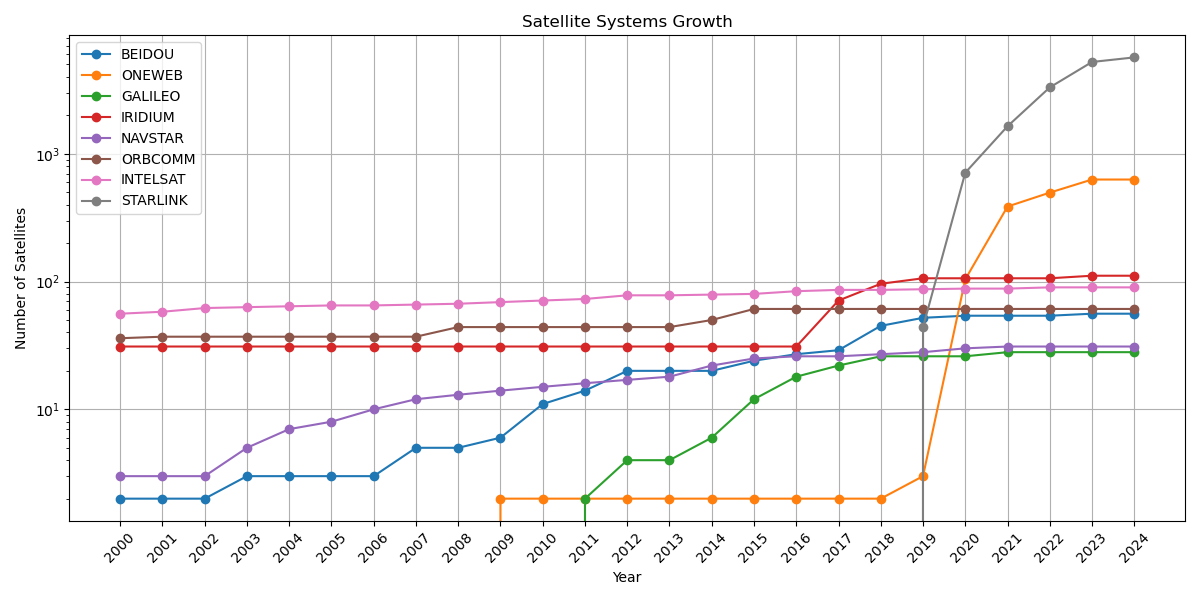
\includegraphics[width=\textwidth]{./chapters/img/satellite-growth.png}
	\caption{Growth of satellite numbers of different satellite constellations since 2000.}
\end{figure}

Therefore, different satellite communication providers (e.g., \textit{Starlink} or \textit{OneWeb}) started constructing their own networked satellite systems.
For different satellite constellations, the development of satellite numbers is shown in Figure~\ref{fig:satellitegrowth}. The numbers originate from N2YO \cite{N2YO2024}, a platform for tracking satellites.

Aside from many previous business failures \cite{Chan2002, Barboza2000}, it is still in question how well networked satellite systems actually work. Previous work reported competitive latencies for \ac{LEO} systems, but increased packet loss \cite{DBLP:conf/imc/MichelTGB22}.
Also, it is in question if networked satellite systems integrate well with existing protocols.



\section{Research Questions} \label{sec:research-questions}

\begin{mdframed}
	\textbf{RQ: How do networked satellite systems perform in terms of latency and packet loss?}
\end{mdframed}

Previous work \cite{DBLP:conf/imc/MichelTGB22, DBLP:conf/infocom/MaCZCML23, Segan2020} showed first results for \ac{RTT} (i.e., latency), throughput, and packet loss. However, networked satellite systems are a cutting edge technology that undergo changes frequently. For example, \cite{DBLP:journals/corr/abs-2403-13497}~et~al. showed a heavily different performance for moving vehicles.
Therefore, it is worth taking a look if significant changes occurred. First, we will have a look on the current performance of networked satellite systems regarding latency and packet loss. Eventually, a system displaying current Starlink performance trends could be developed.

Additionally, we will analyze the Starlink user terminal firmware to evaluate resilience and privacy of the system.

\begin{mdframed}
	\textbf{RQ: How do networked satellite systems perform efficient routing?}
\end{mdframed}

In theory, satellites should integrate well in the existing internet architecture. However, it proved not to be the case. Especially high packet loss \cite{DBLP:conf/infocom/MaCZCML23} poses a problem as a continuous connection cannot be guaranteed.
It should be determined how networked satellite systems currently route packets. That includes considering bent~pipes and ISLs \cite{Hauri2020}.

Ideally, the firmware also allows assessing whether Starlink guarantees privacy and safe data transfer to modern standard of security.
Also, we will explore the limitations of fulfilling the previously mentioned standards in networked satellite systems including \ac{ISLs} and bent pipes.

\begin{mdframed}
	\textbf{RQ: What does the Starlink user terminal firmware reveal about the system's resiliency and privacy?}
\end{mdframed}

The user terminal firmware is a key factor for privacy and resiliency of the Starlink networked satellite system.
Previous attempts in accessing the terminal's built-in firmware were highly successful, but the firmware was not analyzed in detail.

This thesis wants to explore that topic by describing a way to acquire the firmware, describe its structure, and analyze it in regard to resiliency and privacy.




% Background
%	- Networked Satellite Systems
%	- Starlink
%	- Routing: ISLs & Bent-Pipes
\chapter{Background}

\section{Satellite Communication Explained} \label{sec:satellite-communication-explained}

A satellite communication system has the target to send packets from a sender,
connected via a \ac{SNO}, to a receiver connected to a terrestrial ISP.

\begin{figure}[!ht]
	\centering
	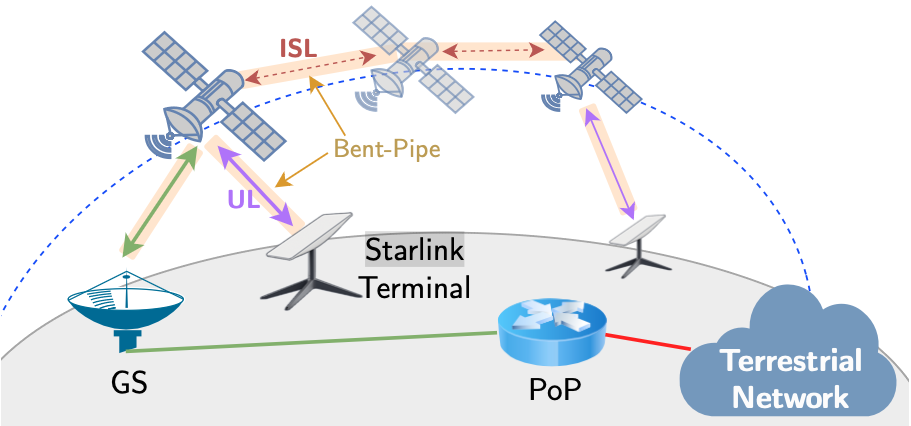
\includegraphics[width=0.7\textwidth]{./chapters/2-background/img/satcom-structure-mohan.png}
	\caption{Schematics of Satellite Communication \cite{DBLP:conf/www/MohanFCBRMO24}.}
	\label{fig:sat-com-explained}
\end{figure}

The structure is illustrated in \Cref{fig:sat-com-explained}. Initially, there
is a sender connected to a satellite antenna provided by the specific \ac{SNO}.
The satellite antenna is also colloquially called "dishy". From the senders'
perspective, there is no different use compared to a traditional terrestrial
internet connection. The antenna sends packets to a satellite that might either
forward the packets to another satellite or directly send them to a nearby
\ac{GS} (also called \ac{PoP}). The \ac{GS} serves as an "entry point" to the
terrestrial internet. A \ac{GS} can forward packets through wired connections,
so they will reach the receiver eventually. \ac{GS}s have to be provided by the
\ac{SNO}. It is essential to have a dense \ac{GS} infrastructure. Fewer
\ac{GS}s can induce higher latencies, as more hops might be necessary.
Therefore, it is necessary to determine an advantageous positioning of \ac{GS}s
\cite{DBLP:conf/sigcomm/VasishtSC21}. For reference, one can get an overview of
current placements of Starlink and OneWeb \ac{GS}s on
\url{https://satellitemap.space}.

The technology of communicating with satellites will not be explained here.
Amongst others, it is described by Pratt~et~al.~\cite{pratt2019satellite}.

Theoretically, the propagation of data in satellite communication happens at
the speed of light. However, the latencies still vary a lot depending on the
choice of \ac{SNO}. Each of them provides a different satellite constellation.
One of the dominating factors is the altitude of the satellites in the
constellation. The higher the satellites are positioned, the more region a
single satellite covers. Therefore, fewer satellites are required to cover a
specific region, which reduces costs. Usually, \ac{SNO}s structure the earth's
surface in cells that receive coverage by at least one satellite. In the case
of Starlink, the world is divided in cells in the form of a hexagon with a
diameter of $\approx 24.13~km$. That translates to a single satellite being
able to cover approximately $379~km^2$ \cite{Pekhterev2021}.

Overall, one differentiates between \ac{GEO} (35'786 km altitude), \ac{MEO}
(2'000 - 35'786 km altitude), and \ac{LEO} (< 2'000 km altitude) satellite
constellations. One can see in \Cref{eq:geo-min-latency} and
\Cref{eq:starlink-min-latency} that this has a significant impact on the
latency.

\begin{equation}
	\frac{2 \cdot 35'786 km}{300'000 \frac{km}{s}} \approx 0.240 s
	\label{eq:geo-min-latency}
\end{equation}
\begin{equation}
	\frac{2 \cdot 550 km}{300'000 \frac{km}{s}} \approx 0.004 s
	\label{eq:starlink-min-latency}
\end{equation}

A \ac{GEO} constellation has a minimum latency of around 240 ms, as shown in
\Cref{eq:geo-min-latency}, assuming a packet needs to reach a satellite in
\ac{GEO} altitude and get back to the earth's surface. On the other hand,
\Cref{eq:starlink-min-latency} shows that a \ac{LEO} satellite constellation at
an altitude of 550 km (like in the case of Starlink) has a minimum latency of
only 4 ms. Research has shown that also in practice \ac{LEO} constellations are
superior compared to \ac{GEO} constellations, especially in terms of latency
\cite{DBLP:journals/pacmnet/RamanVCSZ23, Segan2020}. However, terrestrial
internet still performed better compared to \ac{LEO} constellations
\cite{DBLP:conf/www/MohanFCBRMO24, DBLP:conf/infocom/MaCZCML23}.

\subsection{Bent-Pipes} \label{sec:bent-pipes}

Ground stations are required for satellites to route packets to a receiver.
Depending on the location of the sender, the first satellite on the route might
have to forward packets to a different satellite (using an \ac{ISL}) in order
to reach a region with a \ac{GS}. Such a route is called "Bent-Pipe". Depending
on the number of hops in-between satellites, it is called an "n-hop-bent-pipe".
If the packet needs to be forwarded only once, it is a 1-hop-bent-pipe.

It is in question how bent-pipes influences the performance and behavior of a
networked satellite system. Research still discusses whether bent-pipes provide
a positive (\cite{DBLP:conf/hotnets/HauriBGS20}) or negative
(\cite{DBLP:conf/www/MohanFCBRMO24}) impact.


\section{Use Case of Networked Satellite Systems} \label{sec:usecase-networked-satellite-systems}

The internet has become a key-technology for communication in nearly every
aspect of the society. Having no access to the internet will result in
significant drawbacks. However, internet requires a complex infrastructure with
high cost. Especially in distant location with little population, building such
an infrastructure will not be affordable.

Therefore, people came up with the idea of using satellites to communicate with
distant locations. In theory, only three satellites are required to communicate
with any point on earth (except for polar regions)
\cite{DBLP:conf/5gwf/HofmannK19}. The cost of providing this number of
satellites is much less compared to the costs of providing a terrestrial
network infrastructure with similar accessibility.

There is a group of people that will likely never receive terrestrial network
infrastructure: people on boats and planes. While there is cellular internet
access, it is not offered on the sea and in the high sky. Therefore, the only
option of internet access is satellite internet, which is served all over the
world.

Additionally, networked satellite systems are much more resilient to physical
influences like earthquakes, terrorist attacks, or storms
\cite{DBLP:conf/pam/StevensIBD24}. Terrestrial infrastructure can be destroyed
easily and therefore especially governments contracted networked satellite
system ISPs. A prominent example is the use of Starlink in conflict zones like
Ukraine.

\section{Satellite Network Simulators} \label{sec:satellite_network_simulators}

Amongst concrete measurements, one can also simulate networked satellite
systems. This became increasingly interesting when the constellations were
composed of many more satellites compared to traditional \ac{GEO} satellite
constellations. For example, \ac{LEO} constellations comprise hundreds to
thousands of satellites, which implies a highly complex system.

Sadly, measurements are often highly difficult as they either require acquiring
satellite hardware or recruiting users that already posses the required
hardware. Simulation would tackle both problems, while maintaining low cost. To
the best of our knowledge, we found two networked satellite simulators for
\ac{LEO} constellations.

\subsection{StarPerf} \label{sec:starperf}

\textit{StarPerf}\footnote{\href{https://github.com/SpaceNetLab/StarPerf\_Simulator}{SpaceNetLab/StarPerf\_Simulator}}
\cite{DBLP:conf/icnp/LaiLL20} is a mega-constellation performance simulation
platform. It specifically aims at measuring the impact of the movements of
satellites. Also, it measures performance in different areas. However, setting
it up required, amongst others, Matlab and STK. This made the project difficult
and expensive to test. Therefore, we did not advance in trying out
\textit{StarPerf}.

\subsection{Hypatia} \label{sec:hypatia}

\textit{Hypatia}\footnote{\href{https://github.com/snkas/hypatia}{snkas/hypatia}}
\cite{DBLP:conf/imc/KassingBASS20} is another LEO network simulation framework,
released in 2020 just like \textit{StarPerf}. It aims at a low-level simulation
on packet-level and visualizes the data. Unlike \textit{StarPerf}, it only
requires a Python3 installation. Sadly, running simulations with Hypatia is
highly complex as it requires the user to define, amongst others, the
satellites, ground stations, and points of presence. This information is hardly
available, which renders the simulations barely usable.

\subsection{Problems of Network Simulators}

To the best of our knowledge, research has stopped relying on simulators since
2020. There is proper hardware available that allows testing in the real world.
Testing in the real world has the advantage as it takes more variables into
account. Crucial factors for the performance of a networked satellite system
are the weather, congestion, solar magnetic storms, material failure, and many
more. Those cannot be ideally tested with simulations and will eventually
produce wrong results. Therefore, for further research of this thesis,
simulations will not be used.


% Related Work

% Methodology
%	- Data Sources
%	- Created Data Set
%	- IPInfo
\chapter{Methodology}

\section{Data Collection} \label{sec:data-collection}

For analysis, we create a dataset containing measurements from various sources
about networked satellite systems. Sadly, only data from Starlink devices was
included in the thesis as other \ac{SNO}s did not have sufficient data openly
available.

The data originates from RIPE Atlas, Cloudflare Radar, and N2YO. While
N2YO provides data about satellites, the others hold measurement results. In
the case of N2YO, the website was crawled, while the others provide API
access. The process of data collection is illustrated in
Figure~\ref{fig:data-collection-process}.

\begin{figure}[h]
	\centering
	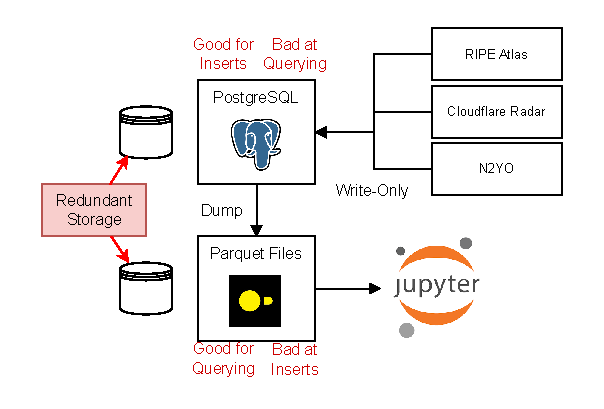
\includegraphics[width=\textwidth]{./chapters/3-methodology/img/architecture.drawio.pdf}
	\caption{Architecture of Data Collection}
	\label{fig:data-collection-process}
\end{figure}

The data is collected from each platform and inserted into a PostgreSQL
database. The database shall allow producers to quickly insert new data (i.e.,
new rows). Transactional databases are the best choice for that, e.g.,
PostgreSQL. To quickly analyze data, an analytical database is the best choice.
For that purpose, Parquet files can be used. Therefore, the data from
PostgreSQL is dumped into the Parquet files. This creates a redundant storage,
in exchange for analysis speed. The resulting data format is shown in
Figure~\ref{fig:er-diagram}.

\begin{figure}
	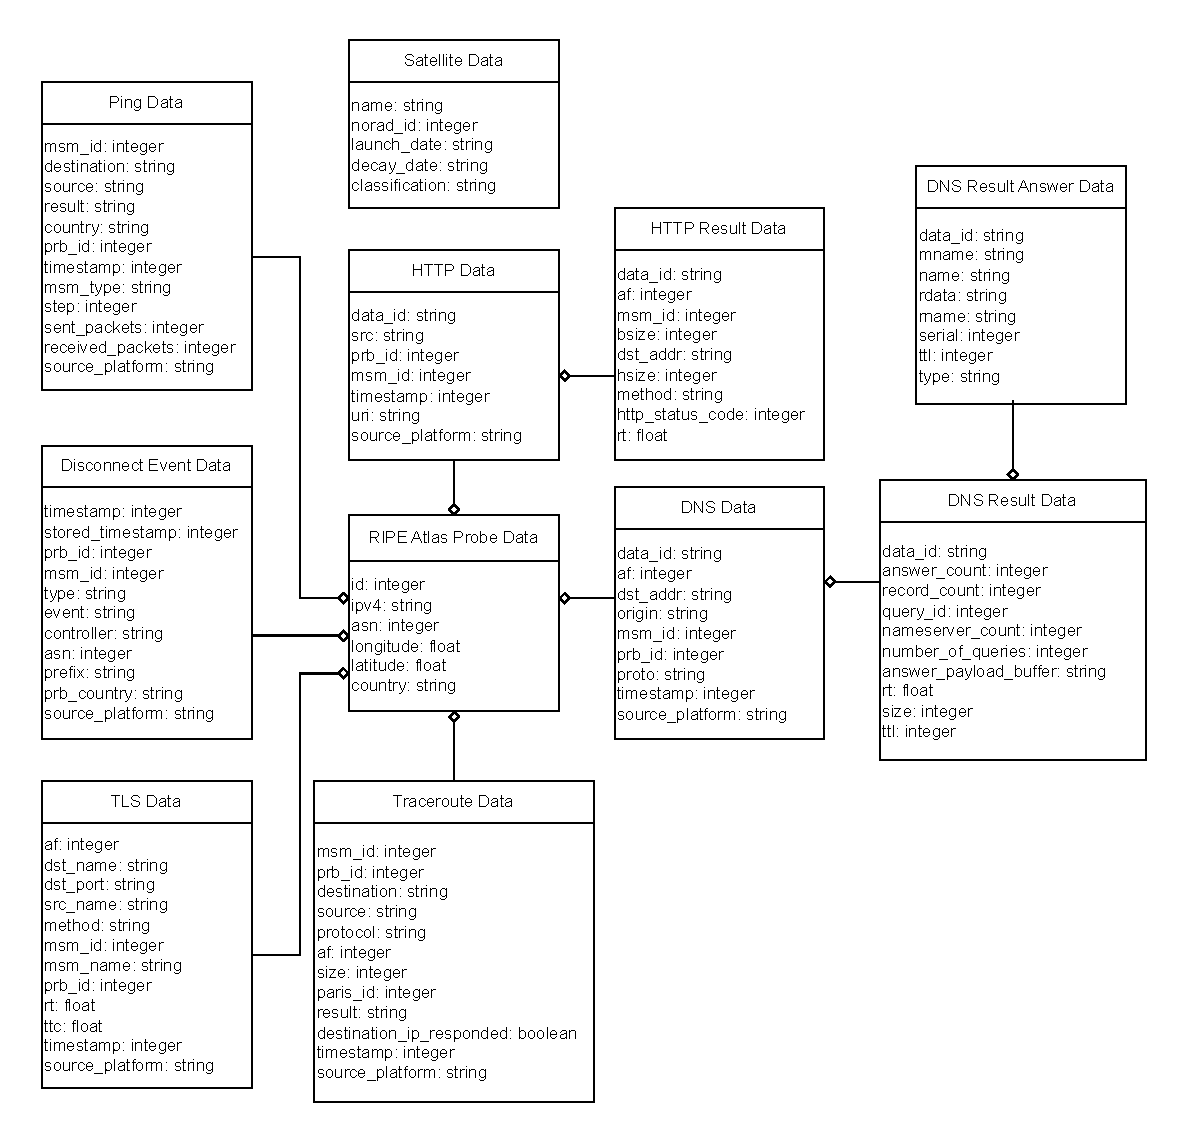
\includegraphics[width=\textwidth]{./chapters/3-methodology/img/er-diagram.drawio.pdf}
	\caption{ER Diagram of Data Schema in PostgreSQL Database.}
	\label{fig:er-diagram}
\end{figure}

The database includes Ping, Traceroute, TLS, HTTP, Disconnect Event, and DNS
measurement data, as well as information about the RIPE~Atlas probes and all
satellites ever launched (including rocket bodies). The whole database
comprises more than 150 GB in PostgreSQL ($\approx$ 50 GB in Parquet files).

Additionally, the measurement data is enriched with data from IPinfo during the
analysis process. However, this data is not included in the dataset and has to
be obtained from IPinfo itself.

\subsection*{RIPE Atlas Data}

RIPE Atlas offers various probes connected via networked satellite systems. At
the moment of writing, all of those probes are connected via Starlink.
Therefore, all the data from RIPE Atlas probes is Starlink data.

Probes are computers running the
\href{https://github.com/RIPE-NCC/ripe-atlas-software-probe}{probe software
	from RIPE Atlas}. They are centrally connected to the RIPE Atlas
servers and
can be used by any person to perform measurements against them. The possible
measurements are defined by the
\href{https://atlas.ripe.net/docs/apis/rest-api-reference/}{RIPE Atlas REST
	API}.

Overall, there are 150 probes from 26 countries. Each probe performs basic
measurements on a regular schedule (so-called built-in measurements). The
built-in measurements are the main source of data and serve as historical
record. This allows to analyze data from 2022. Even if there is Starlink data
prior to 2022, it originates from very little probes and therefore will not be
considered in this thesis to avoid unreliable data.

\section{Reproducibility of Results and Data} \label{sec:reproducibility}

The code to reproduce the results and data is uploaded to GitHub\footnote{See \url{https://github.com/starlink-thesis-diic/starlink-thesis}}. The user is only required to have a running internet connection and an installation of Nix and Docker. Follow the instructions provided by the repository to obtain the results and data by yourself\footnote{The scripts might not work, if data format in the sources has changed since the last update of the scripts.}.


% Results
%	- Packet Loss by Country and Month
%	- Latency by Country and Month
%	- Correlation of Packet Loss and Latency
%	- Routing with Starlink
%	- TODO(robert): What more?
\chapter{results}

% Latency
\section{Latency Development on Individual Days} \label{sec:latency-individual-days}

We used the data to look at the latency development over a single data for individual days.
For that we used the built-in ping measurements taken in RIPE Atlas probes\footnote{Ping measurements are not representative for absolute numbers \cite{DBLP:conf/imc/PelsserCVB13}, but show a pattern.}.


\subsection{Packet Loss from 2022 to 2024} \label{sec:packet-loss}

We looked at the packet loss for the time range from 2022 to June 2024. We use
the Ping measurement from the RIPE Atlas built-in measurements, which by
default send three packets and collect the number of received packets.
Table~\ref{fig:packetloss-total} shows the resulting packet losses in percent
per country.

\begin{table}
	\footnotesize
	\caption{Packet Loss and Latency Correlation in 2022 to June 2024}
	\label{fig:packetloss-total}
	\begin{tabular}{rrlr}
		\toprule
		Sent      & Received  & Country                     & Packet
		Loss Ratio in \%                                             \\
		\midrule
		2150628   & 2134905   & Austria                     & 0.73   \\
		65021654  & 62438854  & Australia                   & 3.97   \\
		22727113  & 22211676  & Belgium                     & 2.27   \\
		1176124   & 1168114   & Benin                       & 0.68   \\
		124263104 & 121160149 & Canada                      & 2.50   \\
		2843      & 2832      & Switzerland                 & 0.39   \\
		3626230   & 3617474   & Chile                       & 0.24   \\
		8092876   & 8074360   & Czechia                     & 0.23   \\
		96089885  & 85983781  & Germany                     & 10.52  \\
		21714610  & 21001677  & Spain                       & 3.28   \\
		432934    & 418925    & Falkland Islands (Malvinas) & 3.24   \\
		321919833 & 299847062 & France                      & 6.86   \\
		83840509  & 80720387  & United Kingdom              & 3.72   \\
		12522224  & 12318835  & Greece                      & 1.62   \\
		271185    & 265100    & Guam                        & 2.24   \\
		18472787  & 18217243  & Haiti                       & 1.38   \\
		37188354  & 35583136  & Italy                       & 4.32   \\
		4160290   & 3829356   & Kiribati                    & 7.95   \\
		127756    & 121937    & Madagascar                  & 4.55   \\
		20450037  & 17548642  & Netherlands                 & 14.19  \\
		26654399  & 21785387  & Philippines                 & 18.27  \\
		18739794  & 18670207  & Poland                      & 0.37   \\
		7047181   & 6967111   & Réunion                     & 1.14   \\
		9975257   & 9922734   & Sweden                      & 0.53   \\
		578852548 & 557475491 & United States               & 3.69   \\
		18571694  & 18463935  & Virgin Islands, U.S.        & 0.58   \\
		\bottomrule
	\end{tabular}
\end{table}

The results are surprising as some countries experience very high packet
losses, while other neighboring countries have rather low packet loss ratios.
For example, Germany and Netherlands are well-developed countries with a
relatively high number of \ac{GS}es. One would expect a low packet loss, which
is not the case. Both countries hold packet loss ratios above ten percent. On
the other hand, neighboring countries like Austria do not show such a pattern.
Another country with remarkably high packet loss are the Philippines, which
have the highest packet loss ratio of all countries.

Overall, most countries experience packet loss ratios at one to four percent,
with some having an even lower value. The lowest value has Czechia with
0.23~\%, while Chile has 0.24~\%.

However, the time range is quite long. Therefore, we looked at the time range
in a more fine-grained interval for the above-mentioned countries.
Figure~\ref{fig:packet-loss-fine-grained} show the packet loss ratios for each
month from January 2022 to June 2024 for Germany, the Netherlands, the
Philippines, and the USA. The first three were chosen as they are noticeable in
Table~\ref{fig:packetloss-total}. The USA was chosen, as it holds the most data
and is therefore a good comparison.

\begin{figure}
	\centering
	\begin{subfigure}[t]{0.47\linewidth}
		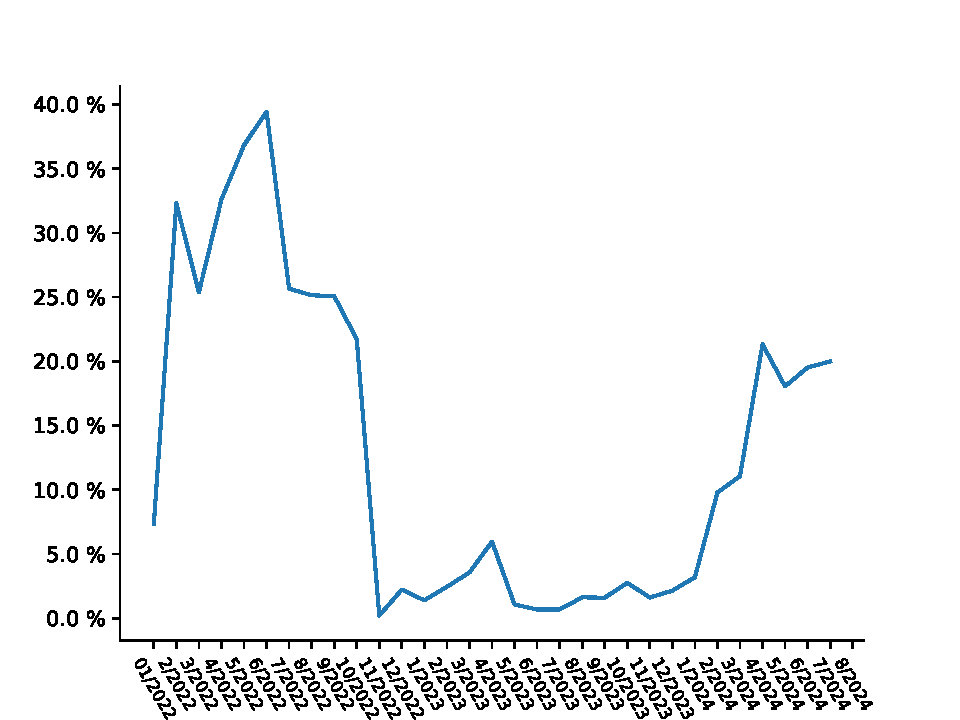
\includegraphics[width=\linewidth]{./chapters/4-results/packet-loss/img/DE.pdf}
		\caption{Germany}
	\end{subfigure}
	\begin{subfigure}[t]{0.47\linewidth}
		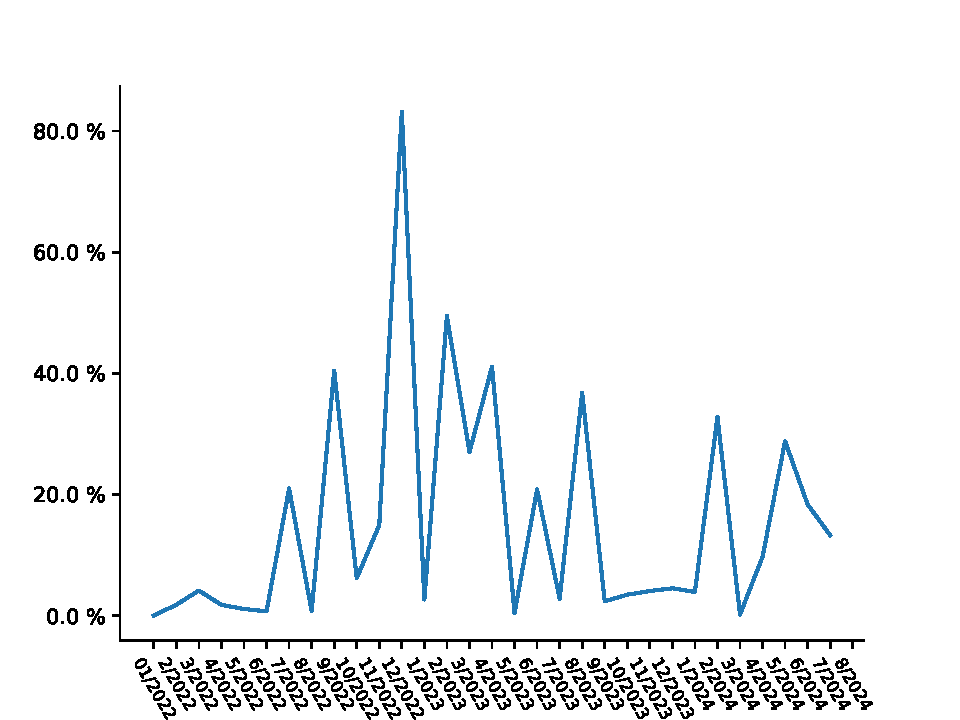
\includegraphics[width=\linewidth]{./chapters/4-results/packet-loss/img/NL.pdf}
		\caption{Netherlands}
	\end{subfigure}
	\begin{subfigure}[t]{0.47\linewidth}
		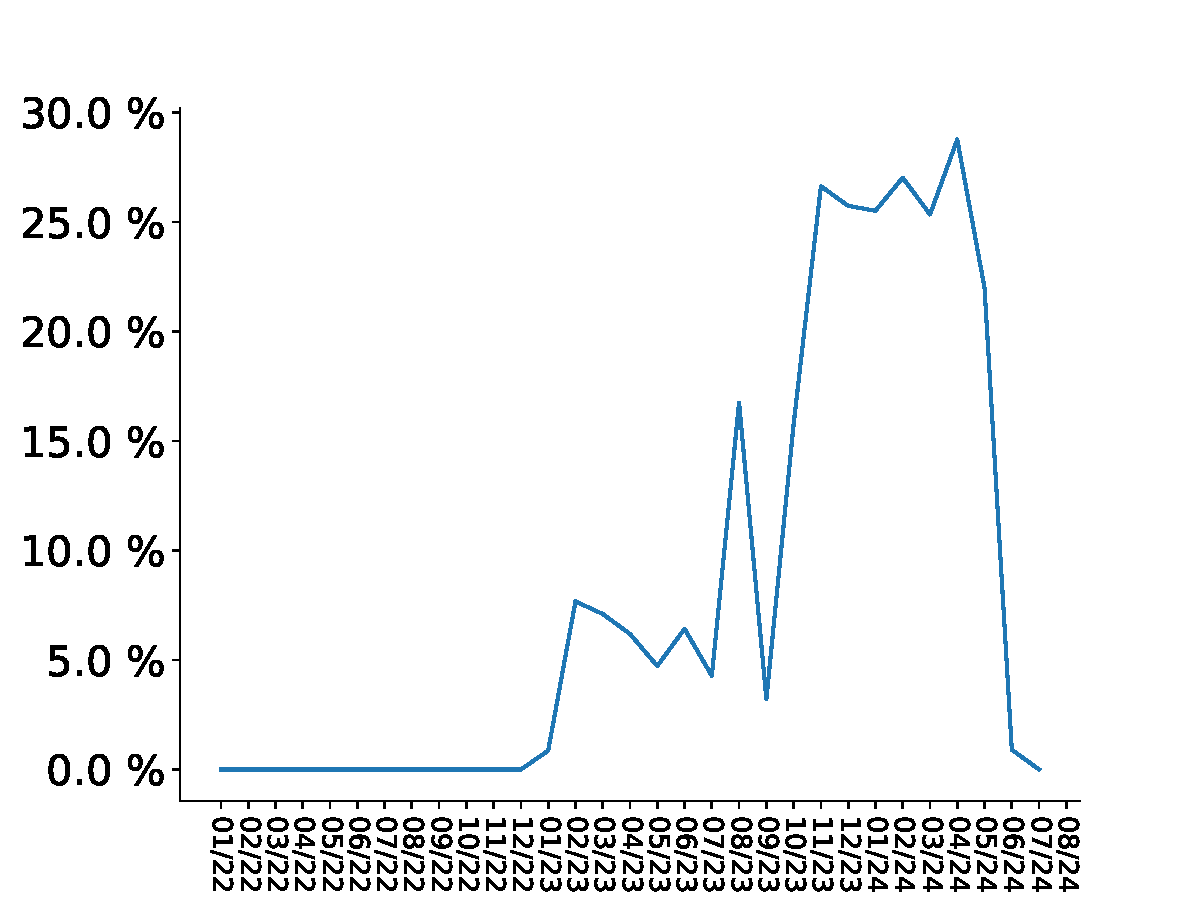
\includegraphics[width=\linewidth]{./chapters/4-results/packet-loss/img/PH.pdf}
		\caption{Philippines}
	\end{subfigure}
	\begin{subfigure}[t]{0.47\linewidth}
		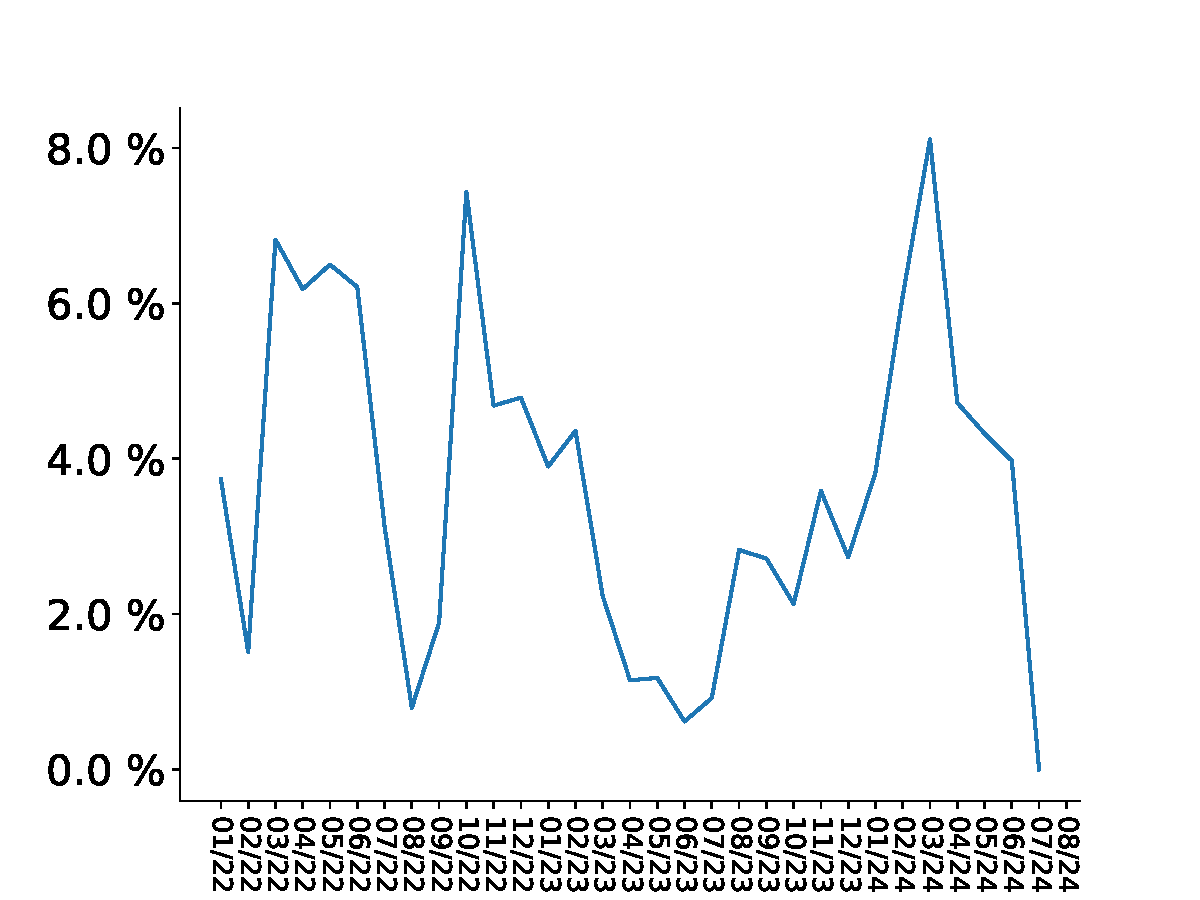
\includegraphics[width=\linewidth]{./chapters/4-results/packet-loss/img/US.pdf}
		\caption{USA}
	\end{subfigure}
	\caption{Packet Loss Ratios in Percent in individual Month from January
		2022 to June 2024}
	\label{fig:packet-loss-fine-grained}
\end{figure}

One can see that Germany experienced high volumes of packet loss in 2022
reaching as high as 40~\% packet loss in June 2022. This was followed by a
period of little packet loss ratios in 2023. Likely, papers taking measurements
at this time will report Germany to have very little packet loss. In 2024, the
trend is going back towards higher packet losses.

The Netherlands show fluctuating pattern that even reaches values of 80~\%
packet loss in December~2022. However, little conclusions can be made except
for the assumption that the connection is highly instable.

The Philippines only hold data since 2023. Therefore, we cannot make
conclusions about the packet loss in the Philippines in 2022. In 2023 however,
the packet loss was around five to eight percent, until in August 2023, the
packet loss rose to more than fifteen percent. In 2024, the packet loss even
rose above twenty-five percent. June 2024 saw a sudden reduction in packet
loss. However, there is to little time series data to determine whether this is
an outlier.

The USA shows a similar pattern to Germany. In 2022, the packet loss was
relatively high, followed by a reducion in 2023, followed by an increase in
2024. However, there are two key differences when comparing Germany and the
USA: (1) the USA experiences lower percentages in packet loss and (2) a
reduction of packet loss is suggested starting in April 2024, which does not
happen for Germany.

\begin{takeaway}{Packet Loss in Starlink}
	The packet loss of Starlink connections is for most countries in the
	range of 1~--~4 \%. However, there are major differences and regional
	proximity does not seem to play a role. Additionally, 2023 has
	experienced better packet loss results compared to 2022 and 2024. This
	is a key difference to the latency analysis, where 2023 has experienced
	the worst results. It seems that Starlink can only op optimize for
	either packet loss and latency. It is in question, whether both values
	correlate.
\end{takeaway}



% Correlation of Packet Loss and Latency
\section{Latency and Packet Loss Correlation} \label{sec:latency-packetloss-correlation}

Latency and packet loss are closely bonded. An increase of packet loss might
yield an increase in latency and vice-versa. For the data presented in the
previous chapter, we looked at the interval from January 2022 to June 2024. For
each month, we used the overall packet loss and the median latency. We used a
Pearson, Kendall, and Spearman correlation to determine possible correlations
between latency and packet loss. The results are shown in
Table~\ref{fig:packetloss-latency-correlation}.

\begin{table}[ht]
	\footnotesize
	\caption{Packet Loss and Latency Correlation}
	\label{fig:packetloss-latency-correlation}
	\begin{tabular}{lrrr}
		\toprule
		Country                     & Pearson     & Kendall     & Spearman    \\
		January 2022 - June 2024    & Correlation & Correlation & Correlation \\
		\midrule
		Falkland Islands (Malvinas) & 0.447641    & 0.595238    & 0.624282    \\
		Réunion                     & 0.636822    & 0.716314    & 0.847658    \\
		Kiribati                    & 0.819596    & 0.794851    & 0.801966    \\
		Canada                      & -0.090981   & 0.218391    & 0.280534    \\
		Poland                      & 0.093155    & -0.025287   & -0.073637   \\
		Haiti                       & 0.383601    & 0.670768    & 0.844964    \\
		Spain                       & -0.323940   & -0.163650   & -0.179434   \\
		Czechia                     & 0.700248    & 0.730392    & 0.806351    \\
		United States               & -0.556997   & -0.425287   & -0.610234   \\
		France                      & 0.893576    & 0.664368    & 0.840267    \\
		Italy                       & -0.073752   & 0.181609    & 0.293882    \\
		United Kingdom              & -0.238013   & -0.227586   & -0.279644   \\
		Honduras                    & 0.415387    & 0.410256    & 0.575585    \\
		Australia                   & -0.025590   & 0.013841    & 0.035834    \\
		Netherlands                 & 0.190923    & 0.055364    & 0.111952    \\
		Greece                      & 0.249727    & 0.496864    & 0.668590    \\
		Sweden                      & 0.678500    & 0.726984    & 0.896199    \\
		Austria                     & 0.054429    & 0.039080    & 0.073192    \\
		Belgium                     & -0.082786   & -0.029885   & -0.031368   \\
		Philippines                 & 0.254523    & 0.460118    & 0.676049    \\
		Virgin Islands, U.S.        & 0.712898    & 0.706384    & 0.878571    \\
		Germany                     & -0.787348   & -0.549425   & -0.753059   \\
		\bottomrule
	\end{tabular}
\end{table}

In a correlation, a value close to 1 or -1 shows a strong correlation. Values
close to 0 do not appear to be correlated. In the results, some countries show
a correlation, e.g., France or Czechia. Other countries, e.g., Canada or
Australia do not show correlating values. As the number of countries with a
stronger and those with a weaker correlation is equally distributed, we cannot
conclude a correlation between latency and packet loss in Starlink networks.

\subsection{Correlation in Single Years}

Analyzing single years give a better understanding of the development of
correlation in the year 2022, 2023, and 2024 (until June). The
Tables~\ref{fig:packetloss-latency-correlation-2022},
\ref{fig:packetloss-latency-correlation-2023}, and
\ref{fig:packetloss-latency-correlation-2024} show the individual correlation
values for the year. There are only countries displayed, where a correlation
value could be calculated.

\begin{table}
	\footnotesize
	\caption{Packet Loss and Latency Correlation in 2022}
	\label{fig:packetloss-latency-correlation-2022}
	\begin{tabular}{lrrr}
		\toprule
		Country        & Pearson     & Kendall     & Spearman    \\
		2022           & Correlation & Correlation & Correlation \\
		\midrule
		Canada         & 0.478988    & 0.272727    & 0.307692    \\
		Poland         & 0.601734    & 0.303030    & 0.342657    \\
		Spain          & -0.286931   & -0.053571   & -0.037594   \\
		United States  & -0.241717   & -0.212121   & -0.363636   \\
		France         & 0.177126    & -0.060606   & -0.083916   \\
		Italy          & 0.646487    & 0.484848    & 0.587413    \\
		United Kingdom & 0.514397    & 0.363636    & 0.496503    \\
		Honduras       & 0.208592    & -0.333333   & -0.426573   \\
		Australia      & 0.870466    & 0.325669    & 0.450715    \\
		Netherlands    & 0.159295    & -0.106873   & -0.164624   \\
		Greece         & 0.811845    & 0.836660    & 0.853766    \\
		Austria        & 0.013609    & -0.060606   & -0.146853   \\
		Belgium        & -0.283806   & -0.242424   & -0.272727   \\
		Germany        & -0.663075   & -0.303030   & -0.517483   \\
		\bottomrule
	\end{tabular}
\end{table}

\begin{table}
	\footnotesize
	\caption{Packet Loss and Latency Correlation in 2023}
	\label{fig:packetloss-latency-correlation-2023}
	\begin{tabular}{lrrr}
		\toprule
		Country                     & Pearson     & Kendall     & Spearman    \\
		2023                        & Correlation & Correlation & Correlation \\
		\midrule
		Falkland Islands (Malvinas) & 0.364389    & 0.466667    & 0.518072    \\
		Réunion                     & 0.587427    & 0.467801    & 0.592125    \\
		Canada                      & 0.370590    & 0.363636    & 0.608392    \\
		Poland                      & -0.261476   & -0.090909   & -0.216783   \\
		Haiti                       & 0.757392    & 0.390673    & 0.529108    \\
		Spain                       & -0.413832   & -0.160714   & -0.218045   \\
		Czechia                     & 0.415844    & 0.383333    & 0.458333    \\
		United States               & -0.302660   & -0.242424   & -0.251748   \\
		France                      & 0.779247    & 0.666667    & 0.818182    \\
		Italy                       & -0.568765   & -0.272727   & -0.412587   \\
		United Kingdom              & -0.812772   & -0.606061   & -0.748252   \\
		Honduras                    & 0.343476    & 0.516667    & 0.617754    \\
		Australia                   & -0.578546   & -0.121212   & -0.258741   \\
		Netherlands                 & 0.212359    & 0.181818    & 0.314685    \\
		Greece                      & -0.268072   & 0.212121    & 0.195804    \\
		Sweden                      & 0.515385    & 0.533333    & 0.717391    \\
		Austria                     & -0.294406   & -0.121212   & -0.125874   \\
		Belgium                     & 0.441123    & 0.454545    & 0.573427    \\
		Philippines                 & -0.196523   & -0.030303   & -0.034965   \\
		Virgin Islands, U.S.        & 0.553108    & 0.578196    & 0.783080    \\
		Germany                     & -0.620018   & -0.424242   & -0.622378   \\
		\bottomrule
	\end{tabular}
\end{table}

\begin{table}
	\footnotesize
	\caption{Packet Loss and Latency Correlation in 2024}
	\label{fig:packetloss-latency-correlation-2024}
	\begin{tabular}{lrrr}
		\toprule
		Country              & Pearson     & Kendall     & Spearman    \\
		2024                 & Correlation & Correlation & Correlation \\
		\midrule
		Réunion              & 0.301680    & -0.066667   & -0.085714   \\
		Kiribati             & 0.744916    & 0.673575    & 0.718421    \\
		Canada               & -0.003851   & -0.600000   & -0.771429   \\
		Poland               & 0.239930    & 0.333333    & 0.371429    \\
		Haiti                & 0.376160    & 0.200000    & 0.257143    \\
		Spain                & -0.044513   & -0.333333   & -0.142857   \\
		United States        & -0.529555   & -0.600000   & -0.771429   \\
		France               & 0.418669    & 0.200000    & 0.257143    \\
		Italy                & -0.600898   & -0.866667   & -0.942857   \\
		United Kingdom       & 0.243811    & 0.333333    & 0.428571    \\
		Honduras             & 0.431954    & 0.333333    & 0.542857    \\
		Australia            & -0.155578   & -0.066667   & -0.085714   \\
		Netherlands          & 0.433624    & 0.466667    & 0.542857    \\
		Greece               & -0.813812   & -0.466667   & -0.600000   \\
		Sweden               & 0.280194    & 0.066667    & 0.085714    \\
		Austria              & 0.915449    & 0.466667    & 0.600000    \\
		Belgium              & 0.428515    & 0.333333    & 0.371429    \\
		Philippines          & -0.920833   & -0.466667   & -0.428571   \\
		Virgin Islands, U.S. & -0.450938   & -0.333333   & -0.428571   \\
		Germany              & -0.603772   & -0.333333   & -0.485714   \\
		\bottomrule
	\end{tabular}
\end{table}

In 2022, there was little correlation at all. Likely, other factors like
satellite infrastructure or presence of \ac{PoP} might have been more
contributing to performance issues. 2023 showed a stronger correlation compared
to 2022. We assume that this is due to a more stable network. The interaction
between packet loss and latency might have become more significant. In 2024,
the correlation decreased once again slightly. This behavior is similar to the
one observed for the latencies in recent months. A possible explanation for
that is a growing user base of Starlink leading to a congestion of the system.
It has to be noted that the growth of number of satellites did not increase
from 2023 to 2024 as much as it did from 2022 to 2023, which might be a cause
of the issue.

\subsection{Correlation with the Number of Probes} \label{sec:number-of-probes-correlation}

It is possible that the data is insufficient resulting in a correlation between
latency and packet loss being invisible. A possibility is to look at the number
of probes being available for each country. Therefore, we took the data from
Table~\ref{fig:packetloss-latency-correlation} and correlated it with the
number of probes available for RIPE Atlas in each country. The resulting table
is shown in Figure~\ref{fig:packetloss-latency-number-probes-correlation}.

\begin{table}[ht]
	\footnotesize
	\caption{Packet Loss, Latency and Number of Probes Correlation}
	\label{fig:packetloss-latency-number-probes-correlation}
	\begin{tabular}{lrrrr}
		\toprule
		Country               & Pearson     & Kendall     & Spearman    & Number of \\
		Jan. 2022 - June 2024 & Correlation & Correlation & Correlation & Probes    \\
		\midrule
		Falkland Islands      & 0.447641    & 0.595238    & 0.624282    & 1         \\
		(Malvinas)                                                                  \\
		Réunion               & 0.636822    & 0.716314    & 0.847658    & 1         \\
		Kiribati              & 0.819596    & 0.794851    & 0.801966    & 2         \\
		Canada                & -0.090981   & 0.218391    & 0.280534    & 11        \\
		Poland                & 0.093155    & -0.025287   & -0.073637   & 1         \\
		Haiti                 & 0.383601    & 0.670768    & 0.844964    & 3         \\
		Spain                 & -0.323940   & -0.163650   & -0.179434   & 4         \\
		Czechia               & 0.700248    & 0.730392    & 0.806351    & 1         \\
		United States         & -0.556997   & -0.425287   & -0.610234   & 53        \\
		France                & 0.893576    & 0.664368    & 0.840267    & 18        \\
		Italy                 & -0.073752   & 0.181609    & 0.293882    & 4         \\
		United Kingdom        & -0.238013   & -0.227586   & -0.279644   & 11        \\
		Honduras              & 0.415387    & 0.410256    & 0.575585    & 1         \\
		Australia             & -0.025590   & 0.013841    & 0.035834    & 8         \\
		Netherlands           & 0.190923    & 0.055364    & 0.111952    & 2         \\
		Greece                & 0.249727    & 0.496864    & 0.668590    & 1         \\
		Sweden                & 0.678500    & 0.726984    & 0.896199    & 1         \\
		Austria               & 0.054429    & 0.039080    & 0.073192    & 4         \\
		Belgium               & -0.082786   & -0.029885   & -0.031368   & 2         \\
		Switzerland           & NaN         & NaN         & NaN         & 1         \\
		Philippines           & 0.254523    & 0.460118    & 0.676049    & 3         \\
		Benin                 & NaN         & NaN         & NaN         & 2         \\
		Virgin Islands, U.S.  & 0.712898    & 0.706384    & 0.878571    & 1         \\
		Germany               & -0.787348   & -0.549425   & -0.753059   & 10        \\
		\bottomrule
	\end{tabular}
\end{table}

We correlated the correlation values with the number of probes per country.
This resulted in the following correlation values:

\begin{itemize}
	\item Pearson Correlation: $\approx -0.44$
	\item Kendall Correlation: $\approx -0.44$
	\item Spearman Correlation: $\approx -0.53$
\end{itemize}

As the correlation does not reach values close to 0, 1, or -1, we cannot
conclude a correlation with the number of probes.

\begin{takeaway}{The correlation of latency and packet loss.}
	Starlink does not show a clear pattern that indicates a correlation
	between latency and packet loss. However, this is highly dependent on
	the country of origin.
\end{takeaway}


% Routing
% last-modified: 08.08.2024
% how-to-reproduce: /src/db-controller/notebooks/traceroute.ipynb

\section{Traceroute Analysis} \label{sec:traceroute-analysis}

Looking at traceroute results, we can make conclusions about the routing behavior of Starlink network devices. In the data we gathered more than forty million traceroute measurements. Those include primarily built-in measurements from RIPE Atlas probes to \textit{*.root-servers.net} for Starlink probes (\ac{ASN} 14593).

\subsection*{Routing Behavior}

\begin{figure}
	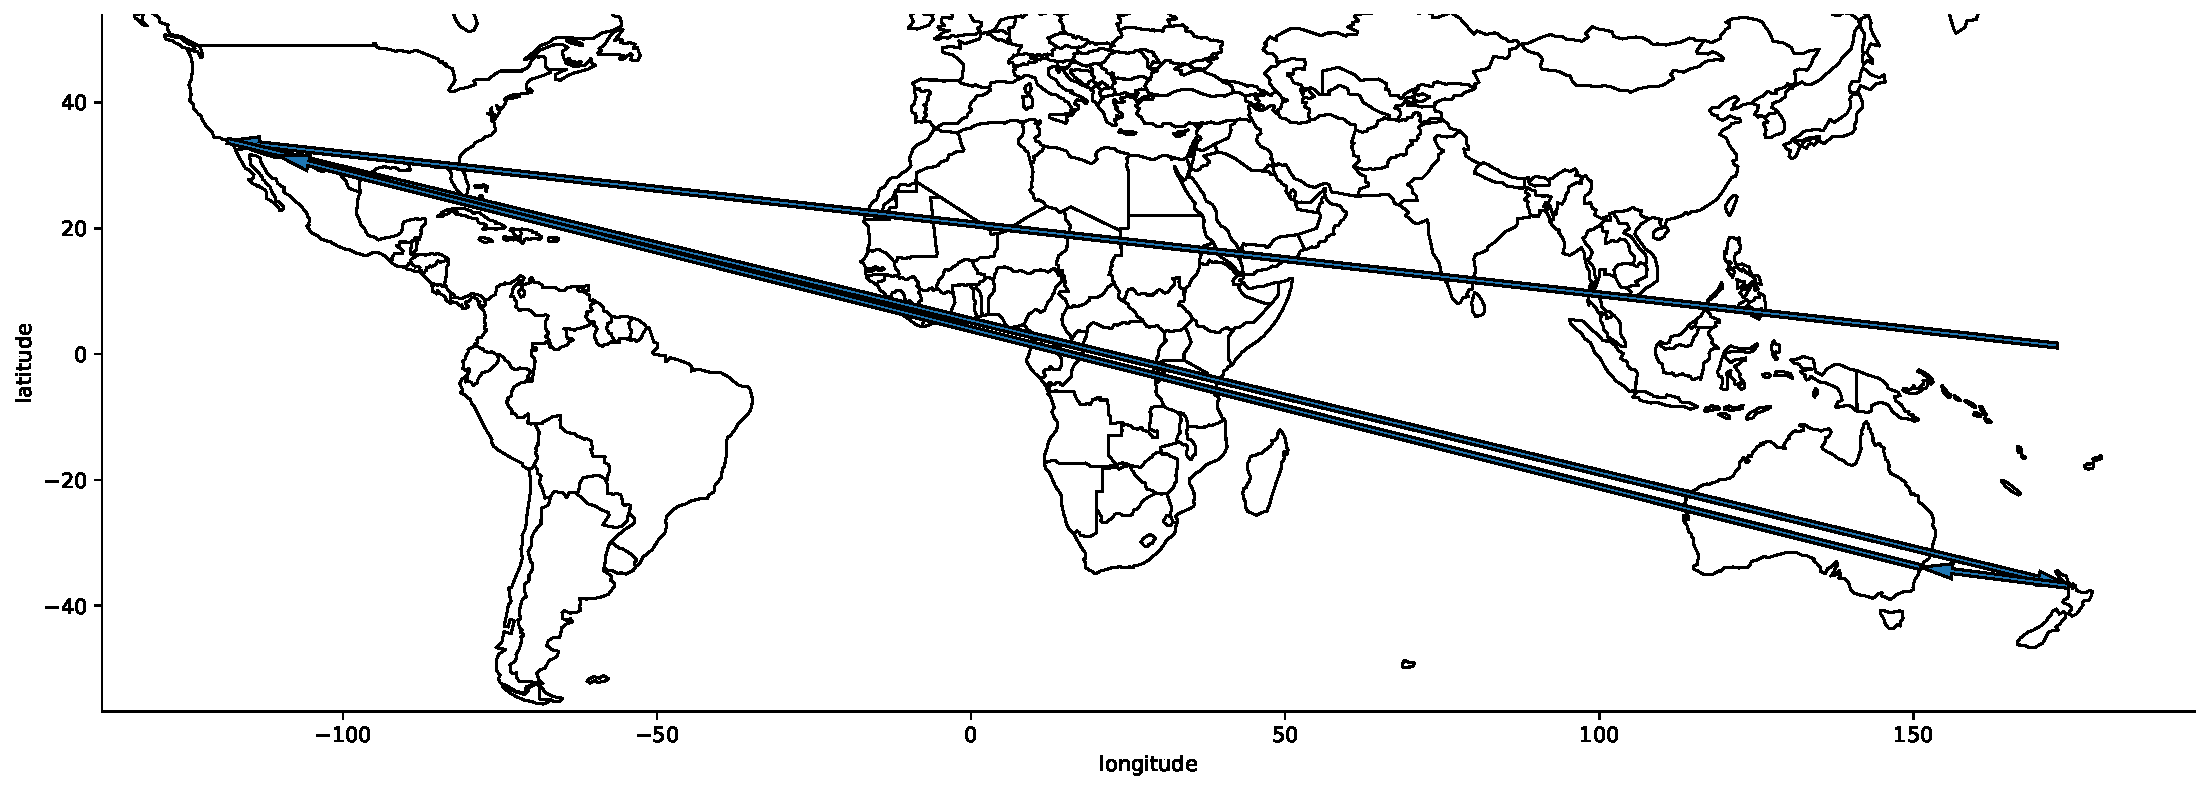
\includegraphics[width=\textwidth]{chapters/4-results/img/kiribati-example-traceroute.pdf}
	\caption{Visualization of a Traceroute from Kiribati}
	\label{fig:kiribati-example-traceroute}
\end{figure}

First, we found that the satellite hops are likely invisible to the traceroute. We conclude that as there are no hops visible above water, even for probes located in remote regions, e.g., Kiribati in the Pacific Ocean. In Figure~\ref{fig:kiribati-example-traceroute}, one can see a visualization of a traceroute result from Kiribati to \textit{f.root-servers.net}. One can see that the first visible hop is located in New~Zealand or an island to the north of New~Zealand. However, if satellites were visible, we'd be able to observe more satellites.

% TODO: Cite the statement that 4000km is too large for a single satellite. Everybody would ask here now: "But how much can they actually cover?"
Coming from the first insight, we can also conclude that \ac{ISLs} are enabled. If they were not, we would likely not be able to see a successful traceroute from Kiribati to a location. The next closest known \ac{PoP} is on Hawaii. However, the distance between both is 4000~km, which is more than a single satellite can cover. Aside from that, we do not observe the usage of the \ac{PoP} in Hawaii, but in more distant locations, which just strengthens the argument. Therefore, we conclude that \ac{ISLs} are enabled. This is special interest, as it was not clear in recent research \cite{Hauri2020}.

\subsection{Privacy Concerns in Traceroute Data}

One of the most important responsibilities of an \ac{ISP} is to ensure the privacy of its users. This also includes to route traffic only in trusted countries. In the case of Starlink, we were able to observe a different behavior. We looked at a slice of the built-in traceroute measurements from German Starlink probes and analyzed their most common targets. We filtered for anycasted servers (e.g., *.root-servers.net) and bogon IPs (i.e., IPs that cannot be associated with metadata).

% Input IP Hitlist
\begin{table}
	\caption{IP Hitlist for Built-In Traceroute Measurements}
	\label{fig:ip-hitlist-traceroute}
	\begin{tabular}{rllll}
		\toprule
		Hits  & City              & Country       & Organization & IP Address      \\
		\midrule
		10634 & Frankfurt am Main & Germany       & AS1299       & 62.115.37.20    \\
		8202  & Offenbach         & Germany       & Unknown      & 80.81.192.154   \\
		6207  & Amsterdam         & Netherlands   & Unknown      & 193.239.116.217 \\
		5582  & Frankfurt am Main & Germany       & AS2914       & 213.198.72.18   \\
		5257  & Frankfurt am Main & Germany       & AS3257       & 89.149.137.14   \\
		4932  & Chicago           & United States & AS14593      & 206.224.65.178  \\
		4916  & Chicago           & United States & AS14593      & 206.224.65.180  \\
		4850  & Chicago           & United States & AS14593      & 206.224.65.182  \\
		4755  & Chicago           & United States & AS14593      & 206.224.65.184  \\
		4358  & Miami             & United States & AS49791      & 81.31.213.126   \\
		4333  & Zürich            & Switzerland   & Unknown      & 185.1.147.30    \\
		4256  & Tokyo             & Japan         & Unknown      & 210.173.176.242 \\
		4179  & Chicago           & United States & AS14593      & 206.224.65.186  \\
		4035  & Chicago           & United States & AS14593      & 206.224.65.192  \\
		4014  & Frankfurt am Main & Germany       & AS6762       & 213.144.184.30  \\
		4010  & Chicago           & United States & AS14593      & 206.224.65.190  \\
		4005  & Chicago           & United States & AS14593      & 206.224.65.188  \\
		4002  & Frankfurt am Main & Germany       & AS1299       & 62.115.124.118  \\
		3990  & Singapore         & Singapore     & AS2497       & 202.232.1.69    \\
		3827  & Frankfurt am Main & Germany       & AS6939       & 72.52.92.70     \\
		\bottomrule
	\end{tabular}
\end{table}

In Table~\ref{fig:ip-hitlist-traceroute}, the top twenty most frequent hits of IP addresses are shown. The IP addresses are joined with data from IPInfo. As traffic goes from a German probe to an anycasted server, located in Germany, one would expect little traffic outside Germany, and none outside Europe. The top five IP addresses are located within or close to Germany, but the next five already involve traffic to the United~States. Here, we observe an unexpected behavior. Assuming that the data is not flawed, this is a clear violation of guiding privacy principles.



% Limitations and Future Work
%	- Limitation of Probe Availability (only selected ones on RIPE Atlas)
%	- Limitation of Service Availability (Starlink only)
%	- Limitation of IPInfo Database
%	- Limitation of Black-Box approach (no insight in Starlink intrinsics)

% Conclusion

% Reproducability Considerations
